\subsection{RadixVM: Scalable address space operations}

\XXX![AC]{Introduce: ``The virtual memory interface is rife with
  commutativity, but existing implementations scale very poorly.''
  Pull in some of the EuroSys design section intro.}

\XXX![AC]{This uses subsubsections, but \refcache uses paragraphs.}

\XXX![AC]{Below here this section is verbatim from the EuroSys paper.
  Flow into thesis.}

\subsubsection{Radix tree}
\label{sec:radixvm:tree}

At its core, an address space is a mapping from virtual addresses to
metadata and physical memory.  To achieve perfectly scalable
non-overlapping address space operations, \vm needs a data structure
that can track this mapping and support \code{mmap}ing and
\code{munmap}ing ranges of virtual address space while avoiding
contention between operations on disjoint regions.

One option to avoid contention is to avoid sharing altogether. For
example, one could attempt to partition the address space of a process
statically
among the cores, and have each core manage its part of the address space.
This option ensures that operations on non-overlapping memory regions
that are in different partitions of the address space don't contend
for cache lines because each region is in a different partition. The
downside of this option is that static partitioning complicates
sharing and requires the application developer to
be aware of the partitioning, so that each thread manipulates
regions that are in its partition.  A more desirable solution is
to use some shared data structure that allows symmetric operations
from all threads to manage the shared address space,
as all current VM systems do.

In particular, a data structure that supports lock-free operations---such
as the Bonsai tree does for read
operations~\cite{clements:bonsai}---seems promising, since it avoids
cache line contention due to locks.  Lock-free operation,
however, doesn't imply \emph{no} cache line contention.  For example,
\code{insert} and \code{lookup} operations for a lock-free concurrent skip
list~\cite{herlihy:art} can result in contention for cache lines
storing interior nodes in the skip list---even when the \code{lookup}
and \code{insert} involve different keys---because \code{insert} must
modify interior nodes to maintain $O(\log n)$ lookup time.  As we will show
in \S\ref{sec:eval}, this read-write sharing scales badly with more cores,
as more cores need to reread cache lines modified by unrelated
operations on other cores.

Any balanced tree or similar data structure suffers from this unintended
cache line contention.  A (completely impractical) strawman solution is
to represent a process's virtual memory by storing the metadata for each
virtual page individually in a large linear array indexed by virtual
page number.  In this linear representation, \code{mmap}, \code{munmap},
and \code{pagefault} can lock and manipulate precisely the pages being
mapped, unmapped, or faulted.  VM operations on non-overlapping
memory regions will access disjoint parts of the linear array
and thus scale perfectly.  The design presented in this section follows
the same general scheme as this strawman design, but makes its memory
consumption practical using a multilevel, compressed radix tree.

\begin{figure}
\centering
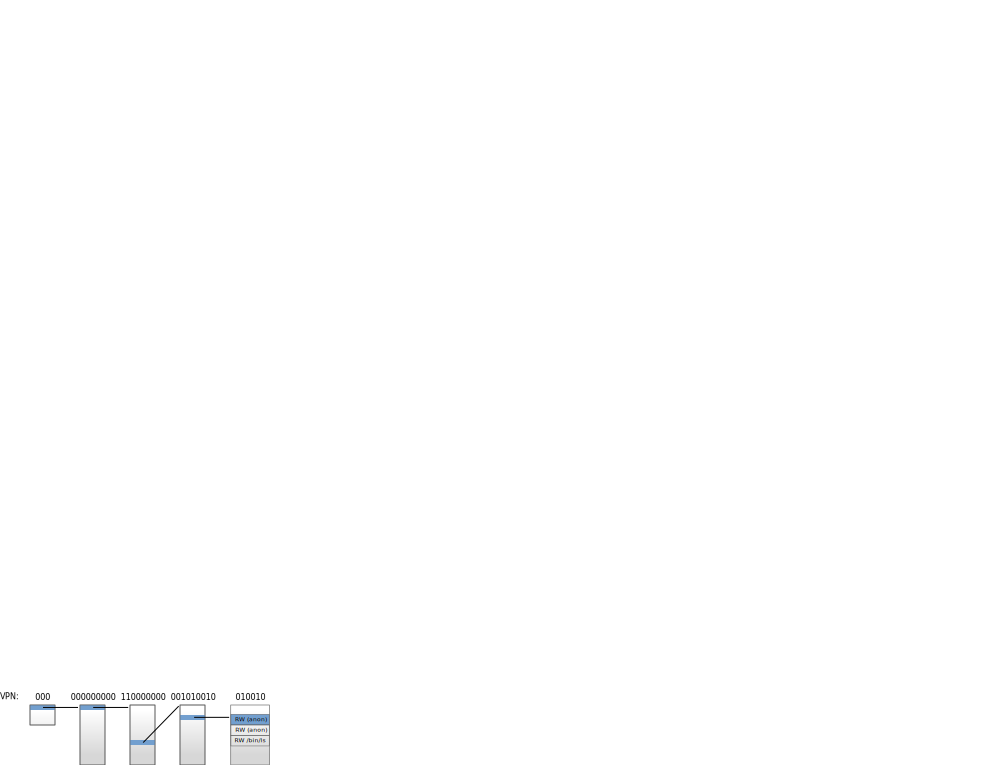
\includegraphics{figures/radix.pdf}
\caption{A radix tree containing both an anonymous mapping
  and a file mapping.  Blue indicates the path for looking up the 36-bit
  virtual page number shown in bits at the top of the figure.  The last
  level of the tree contains separate mapping metadata for each page.
}
\label{fig:radix}
\end{figure}

The index data structure of \vm resembles a hardware page table
structurally, storing mapping metadata in a fixed-depth radix tree,
where each level of the tree is indexed by nine (or fewer) bits of the
virtual page number (Figure~\ref{fig:radix}).  Like the linear array,
the radix tree supports only point queries (not range queries) and
iteration, but unlike the linear array, \vm can compress repeated
entries and lazily allocate the nodes of the radix tree.  Logically,
any node that would consist entirely of identical values is folded
into a single value stored in the parent node.  This continues up to
the root node of the tree, allowing the radix tree to represent vast
swaths of unused virtual address space with a handful of NULL values
and to set large ranges to identical values very quickly.  This
folding comes at a small cost: \code{mmap} operations that force
expansion of the radix tree may conflict with each other, even if
their regions do not ultimately overlap.  However, such conflicts are
rare.

To record each mapping, \vm stores a separate copy of the mapping metadata
in the radix tree for each page in the mapped range.  This differs
from a typical design that allocates a single metadata object
to represent the entire range of a mapping (e.g., virtual memory areas
in Linux).
Storing a separate copy of the metadata for each page makes sense in \vm
because the metadata is relatively small, and eliminating shared objects
avoids contention when a single mapping needs to be split or merged by
a subsequent \code{mmap} or \code{munmap} call.  Furthermore, the
mapping metadata object is designed so that it will initially be
identical for every page of a mapping, meaning that large mappings can
created efficiently and folded into just a few slots in the radix
tree's nodes.

Also unlike typical virtual memory system designs, \vm stores pointers
to physical memory pages in the mapping metadata for pages that have
been allocated.  This is easy to do in \vm because, modulo folding,
there is a single mapping metadata object for each page.  It's also
important to have this canonical representation of the physical memory
backing a virtual address space because of the way \vm handles TLB
shootdown (see \S\ref{sec:radixvm:tlb}).  This does increase the space
required by the radix tree, but, asymptotically, it's no worse than
the hardware page tables, and it means that the hardware page tables
themselves are cacheable memory that can be discarded by the OS to
free memory.

To keep the memory footprint of the radix tree in check, the OS must be
able to free nodes that no longer contain any valid mapping metadata.
To accomplish this without introducing contention, we leverage
\refcache to scalably track the number of used slots in each node.
When this count drops to zero, the radix tree can remove the node from
the tree and delete it.  Since \vm may begin using a node again before
\refcache reconciles the used slot count, nodes link to their children
using weak references, which allows the radix tree to revive nodes
that go from empty to used before \refcache deletes them, and to
safely detect when an empty child node has been deleted.

Collapsing the radix tree does introduce additional contention;
however, in
contrast with more eager garbage collection schemes, rapidly changing
mappings cannot cause the radix tree to rapidly delete and recreate
nodes.  Since a node must go unused for at least two \refcache epochs
before it is deleted, any cost of deleting or recreating it (and any
additional contention that results) is amortized.
\XXX[AC]{We don't actually implement this, but if we did, when we
analyze performance without \refcache, things would be even worse.
Might be worth mentioning.}

In contrast with more traditional balanced trees, using a radix tree
to manage address space metadata allows \vm to achieve perfect
scalability for operations on non-overlapping ranges of an address
space.  This comes at the cost of a potentially larger memory
overhead; however, address space layouts tend to exhibit good
locality and folding efficiently compresses large ranges, making radix
trees a good fit for a VM system.

\subsubsection{TLB shootdown}
\label{sec:radixvm:tlb}

One complication with scaling \code{mmap} or \code{munmap} operations
is the per-core hardware page translation cache, which requires
explicit notifications (``TLB shootdowns'') when a page mapping changes.
Because TLB shootdowns must be delivered to every CPU that may have
cached a page mapping that's being modified, and because hardware does not provide
information about which CPUs may have cached a particular mapping,
a conservative design must send TLB shootdown interrupts to all
CPUs using the same address space, which limits scalability.

\vm achieves better scalability for \code{mmap} and \code{munmap} by
keeping track of more precise information about the set of CPUs that
may have accessed a given mapping, as part of the mapping metadata.
With a software-filled TLB, the kernel can use TLB miss faults to track
exactly which CPUs have a given mapping cached.  When a later \code{mmap}
or \code{munmap} changes this mapping, it can deliver shootdowns
only to cores that have accessed this mapping.  On architectures
with hardware-filled TLBs such as the x86, our design achieves the
same effect using per-core page tables.  If a thread in an application
allocates, accesses, and frees memory on one core, with no other threads
accessing the same memory region, then \vm will perform no TLB shootdowns.

The obvious downside to this approach is the extra memory required for
per-core page tables.  We show in \S\ref{eval:memory} that this
overhead is small in practice compared to the total memory footprint
of an application, but for applications with poor partitioning, it may
be necessary for the application to provide hints about widely shared
regions so the kernel can share page tables (similar to Corey address
ranges~\cite{boyd-wickizer:corey}) or
the kernel could detect such regions automatically.  The kernel could
also reduce overhead by sharing page tables between small groups of
cores or by simply
discarding page table pages when memory is low.

\subsubsection{VM operations}

The POSIX semantics of VM operations can make a scalable implementation
of the operations challenging~\cite{clements:bonsai}. But, with the
components described above, the \vm implementation of the VM operations is
surprisingly straightforward.  The POSIX semantics that are challenging
are the ones that relate to ordering. For example, after the return
of an \code{munmap}, no thread should be able to access the unmapped
pages.  Similarly, after \code{mmap}, every thread that experiences a
\code{pagefault} should be able to access the mapped pages.  There is
also some
complexity in \code{pagefault} because it is not just a read operation:
it may have to allocate physical pages and modify the address space.

\vm primarily enforces correct ordering semantics by always locking,
from left to right, the radix tree entries for the region affected by
an operation.  Each slot in the radix tree (in both interior and leaf
nodes) reserves one bit for this purpose.  As a result, two concurrent
VM operations on overlapping ranges will serialize when locking the
leftmost overlapping page.

When locking a region that has not been expanded out to leaf nodes
yet, \vm acquires locks on the corresponding internal node slots instead.
When \vm expands the tree by allocating new nodes, it propagates the
lock bit to every entry in the newly allocated node, and unlocks the
parent interior node slot.  Releasing the lock clears the lock bits in the
newly allocated child node.  Tree traversal does not require locks
because it increments each node's reference count through a \refcache
weak reference.

An \code{mmap} invocation first locks the range being mapped.  As above,
if the leaf nodes for the range have already been allocated, \code{mmap}
locks the mapping metadata in the leaf nodes, and if not, it locks the
corresponding interior nodes.  If there are existing mappings within the
range, \code{mmap} unmaps them, as described later for \code{munmap}.
\code{mmap} then fills in mapping metadata for the new mapping (protection
level and flags arguments to \code{mmap}, as well as what backs this virtual
memory range, such as a file or anonymous memory).  If the mapping covers
an entire radix tree node, and the child nodes have not been allocated
yet, the radix tree collapses the mapping metadata into a single slot
in the interior of the tree.
Otherwise, \vm copies the mapping metadata into each leaf node entry in
the range.  Finally, \vm unlocks the range.  Like in other VM systems,
\code{mmap}
doesn't allocate any physical pages, but leaves that to \code{pagefault},
so that pages are allocated only when they are used.

A \code{pagefault} invocation traverses the radix tree to find the
mapping metadata for the faulting address, and acquires a lock on it.
It then allocates a physical page, if one has not been allocated yet, and
stores it in the mapping metadata.  Finally, \code{pagefault} fills in the
page table entry in the local core's page table, and adds the local core
number to the TLB shootdown list in the mapping metadata for that address.
\code{pagefault} then releases the lock and returns.

To implement \code{munmap}, \vm must clear mapping metadata from the
radix tree, clear page tables, invalidate TLBs, and free physical
pages.  \code{munmap} begins by locking the range being unmapped,
after which it can scan the region's metadata to gather references to
the physical pages backing the region, collect the set of cores that
have faulted pages in the region into their per-core page tables, and
clear each page's metadata.  It can then send inter-processor
interrupts to the set of cores it collected in the first step.  These
interrupts cause the remote cores (and the core running \code{munmap})
to clear the appropriate range in their per-core page table and
invalidate the corresponding local TLB entries.  Once all cores have
completed this shootdown process, \code{munmap} can safely release its
lock on the range and decrement the reference counts on the physical
pages that were unmapped.

Note that an invocation of \code{pagefault} on one core may concurrently
access a page that another core is in the process of unmapping,
but the mapping metadata lock makes this work out correctly: either
\code{pagefault} acquires the lock first or \code{munmap} does.  In the
first case, the page fault succeeds, which is okay since the pages must be
inaccessible only after \code{munmap} returns.  In the second case, the
\code{munmap} runs first and removes the mapping for the unmapped range
before releasing the locks. Then, \code{pagefault} will see that there
is no mapping for the faulting address and will halt the faulting thread.

\subsubsection{Discussion}

By combining \refcache for scalable reference counting, radix trees
for maintaining address space metadata, and per-core page tables for
precise TLB tracking and shootdown, \vm is able to execute concurrent
\code{mmap}, \code{munmap}, and \code{pagefault} operations on the
same address space in a way that shares cache lines only when two operations
manipulate overlapping regions and must be serialized.  With the right
data structures in place, \vm can achieve this with a straightforward
concurrency plan based on precise range locking.  We confirm that
\vm's design translates into scalable performance for non-overlapping
VM operations in \S\ref{sec:eval}.

